\documentclass[../main.tex]{subfiles}

\begin{document}

  \subsection*{Limits at Infinity}
  \begin{definition}
    We will say that $\lim_{x \to \infty} f(x)=L$ if $f(x)$ is ``close enough'' to $L$ whenever $x>0$ is ``large enough''.

    Similarly we define $\lim_{x \to -\infty} f(x) = L$ if $f(x)$is ``close enough'' to $L$ whenever $x<0$ is ``large enough''.

    If either $\lim_{x \to \infty} f(x)=L$ or $\lim_{x \to -\infty} f(x)=L$, we say that the line $y=L$ is an \textbf{horizontal asymptote} of the graph of $f$.
  \end{definition}

  \begin{example}
    Argue that
    \[
      \lim_{x \to \infty} 1/x = \lim_{x \to \-\infty} 1/x = 0.
    \]
    by making a table of values of $x$ and $1/x$.

    \begin{figure}[H]
      \centering
      \begin{tikzpicture}
\begin{axis}%
    [
        title={$f(x) = \dfrac{1}{x}$},
        grid=major,
        x=2mm,
        y=2mm,
        xmin=-10,
        xmax=10,
        xlabel={$x$},
        axis x line=middle,
        ymin=-10,
        ymax=10,
        axis y line=middle,
        no markers,
        samples=100,
        domain=-10:10
    ]
    \addplot[thick,samples=400] (x,{1/x});
\end{axis}
\end{tikzpicture}
    \end{figure}
  \end{example}
  Recall that for ordinary limits, limit of product of functions is a product of limits of functions. Same is also true for limits at infinity. Hence
  \[
    \lim_{x \to \infty} \frac{1}{x^2} =
    \lim_{x \to \infty} \frac{1}{x}  \cdot \lim_{x \to \infty} \frac{1}{x}  = 0 \times 0 = 0.
  \]

  Similarly
  \[
    \lim_{x \to -\infty} \frac{1}{x^2} = 0
  \]

  Finally, for any positive integer $n$
  \[
    \lim_{x \to \infty} \frac{1}{x^n} =
    \lim_{x \to -\infty} \frac{1}{x^n} = 0.
  \]

  \begin{figure}[H]
    \centering
    \begin{tikzpicture}
  \begin{axis}[
    title={$f(x)=\dfrac{x}{\sqrt{x^2+1}}$},
    grid=major,
    axis lines = middle,
    ymax=1.2,
    ymin=-1.2,
    xlabel={$x$},
    ylabel={$y$},
    scale=.6
  ]
  \addplot[domain=-6:6, samples=400, thick] {x/sqrt(x^2+1)};
  \end{axis}
\end{tikzpicture}
  \end{figure}
  \begin{example}
    Let $f(x)=\dfrac{x}{\sqrt{x^2+1}}$. Find $\lim_{x \to \infty} f(x)$, $\lim_{x \to -\infty} f(x)$.
  \end{example}
  \begin{solution}
    \[
      \begin{split}
        \lim_{x \to \infty} \dfrac{x}{\sqrt{x^2+1}} & =
        \lim_{x \to \infty} \dfrac{x}{\abs{x}\sqrt{1+1/x^2}} =
        \lim_{x \to \infty} \dfrac{x}{x \sqrt{1+1/x^2}} =
        \lim_{x \to \infty} \dfrac{1}{\sqrt{1+1/x^2}} =
        \dfrac{\lim_{x \to \infty} 1}{\lim_{x \to \infty} \sqrt{1+1/x^2}} \\
        & = \dfrac{1}{\sqrt{\lim_{x \to \infty} (1+1/x^2)}} =
        \dfrac{1}{1} = 1.
      \end{split}
    \]
    Similarly,
    \[
      \lim_{x \to -\infty} \dfrac{x}{\sqrt{x^2+1}} = -1
    \]
  \end{solution}

  \subsection*{Limits of Rational Functions at Infinity}
  Recall that a rational function is a ratio of two polynomials.

  \textit{Strategy.} To find limits of rational functions at infinity, divide by the highest power of $x$ appearing in the \textit{denominator}.

  \begin{example}
    \[
      \lim_{x \to \pm \infty} \frac{2x^2-x+3}{3x^2+5} =
      \lim_{x \to \pm \infty} \frac{2-\frac{1}{x} + \frac{3}{x^2}}{3+\frac{5}{x}} = \frac{2}{3}.
    \]
  \end{example}

  \begin{example}
    \[
      \lim_{x \to \pm \infty} \frac{x-5}{2x^2+4x+1} =
      \lim_{x \to \pm \infty} \frac{\frac{1}{x}-\frac{5}{x^2}}{2+\frac{4}{x}+\frac{1}{x^2}} = \frac{0}{2} = 0.
    \]
  \end{example}

  We can generalize the above examples.
  \begin{theorem}
    Let $P(x) = a_p x^p + a_{p-1} x^{p-1} + \dots + a_0$ be a polynomial of degree $p$ and $Q(x) = b_q x^q + \dots + b_0$ be a polynomial of degree $q$.
    If $p = q$, then
    \[
      \lim_{x \to \pm \infty} \frac{P(x)}{Q(x)} = \frac{a_p}{q_p},
    \]
    If $p<q$, then
    \[
      \lim_{x \to \pm \infty} \frac{P(x)}{Q(x)} = 0,
    \]
  \end{theorem}

  \begin{example}
    \[
      \lim_{x \to \infty} \sqrt{x^2+x} - x =
      \lim_{x \to \infty} \frac{(\sqrt{x^2+x} - x)(\sqrt{x^2+x} + x)}{\sqrt{x^2+x} + x} =
      \lim_{x \to \infty} \frac{x}{\abs{x}\sqrt{1+\frac{1}{x}} + x} =
      \lim_{x \to \infty} \frac{1}{\sqrt{1+\frac{1}{x}} + 1} = \frac{1}{2}.
    \]
  \end{example}

  \subsection*{Infinite Limits}
  \begin{example}
    The values of $\dfrac{1}{x^2}$ gets larger and larger as $x$ approaches to 0. Thus $\lim_{x \to 0} \dfrac{1}{x^2}$ does not exist. Although the limit does not exist, it is useful to state why it does not exist by writing
    \[
      \lim_{x \to 0} \frac{1}{x^2} = \infty.
    \]

    \begin{figure}[H]
      \centering
      \begin{tikzpicture}
\begin{axis}%
    [
        title={$f(x) = \dfrac{1}{x^2}$},
        grid=major,
        x=2mm,
        y=2mm,
        xmin=-10,
        xmax=10,
        xlabel={$x$},
        axis x line=middle,
        ymin=-10,
        ymax=10,
        axis y line=middle,
        no markers,
        samples=100,
        domain=-10:10
    ]
    \addplot[thick,samples=400] (x,{1/(x^2)});
\end{axis}
\end{tikzpicture}
    \end{figure}
  \end{example}

  \begin{example}
    \[
      \lim_{x \to 0+} \frac{1}{x} = \infty.
    \]
    \[
      \lim_{x \to 0-} \frac{1}{x} = -\infty.
    \]
    \[
      \lim_{x \to 0} \frac{1}{x} \text{ does not exist}.
    \]
  \end{example}

  \begin{example}
    \[
      \lim_{x \to -\infty} \sqrt{x^2+x} - x =
      \lim_{x \to -\infty} \frac{(\sqrt{x^2+x} - x)(\sqrt{x^2+x} + x)}{\sqrt{x^2+x} + x} =
      \lim_{x \to -\infty} \frac{x}{\abs{x}\sqrt{1+\frac{1}{x}} + x} =
      \lim_{x \to -\infty} \frac{1}{-\sqrt{1+\frac{1}{x}} + 1}
    \]

    If $x<0$ then $\sqrt{1+\frac{1}{x}}<1$ and $-\sqrt{1+\frac{1}{x}} + 1 >0$. Hence the denominator is positive and approaches to zero. So
    \[
      \lim_{x \to -\infty} \frac{1}{-\sqrt{1+\frac{1}{x}} + 1} = \infty.
    \]
  \end{example}

  \subsection*{Behaviour of Polynomials at Infinity}
  \begin{example}
    \[
      \lim_{x \to \infty} 4x^3 - 2x + 1 =
      \lim_{x \to \infty} 4x^3 = \infty.
    \]

    \[
      \lim_{x \to -\infty} -3x^5 + x^3 +1 =
      \lim_{x \to -\infty} -3 x^5 = \infty.
    \]
  \end{example}
  In general,
  \begin{theorem}
    If $P(x) = a_n x^n + \cdots + a_0$ is a polynomial then
    \[
      \lim_{x \to \pm \infty} P(x) = \lim_{x \to \pm \infty} a_n x^n.
    \]
  \end{theorem}

  \begin{example}
    \[
      \lim_{x \to \infty} \frac{x^3+1}{x^2-2x} =
      \lim_{x \to \infty} \frac{x+\frac{1}{x^2}}{1-\frac{2}{x}} = \lim_{x \to \infty} \frac{x}{1} = \infty
    \]
  \end{example}

  \begin{example}
    \begin{enumerate}
      \item $\lim_{x \to 2} \dfrac{(x-2)^2}{x^2-4} = 0$
      \item $\lim_{x \to 2+} \dfrac{x-3}{x^2-4} = -\infty$
      \item $\lim_{x \to 2-} \dfrac{x-3}{x^2-4} = \infty$
      \item $\lim_{x \to 2} \dfrac{x-3}{x^2-4}$ does not exist.
      \item $\lim_{x \to \infty} \dfrac{2x-1}{\sqrt{3x^2+x+1}}$,
      \item $\lim_{x \to 1+} \dfrac{\sqrt{x^2-x}}{x-x^2}$
      \begin{solution}
        If $x>1$ then $x-x^2 = x(1-x) < 0$. So
        \[
          \lim_{x \to 1+} \dfrac{\sqrt{x^2-x}}{x-x^2} =
          \lim_{x \to 1+} \dfrac{-\sqrt{x^2-x}}{x^2-x} =
          \lim_{x \to 1+} \dfrac{-\sqrt{x^2-x}}{\sqrt{x^2-x} \sqrt{x^2-x}} =
          \lim_{x \to 1+} \dfrac{-1}{\sqrt{x^2-x}} = -\infty
        \]
      \end{solution}
    \end{enumerate}
  \end{example}
\end{document}